\documentclass[a4paper,12pt]{article}
\usepackage{titlesec}
\usepackage{indentfirst}
\usepackage{graphicx}
\usepackage{amsmath}
\usepackage{float,subcaption}
\usepackage[hidelinks]{hyperref}

\graphicspath{ {./img/} }

\newcommand{\sectionbreak}{\clearpage}

\begin{document}

	\begin{titlepage}
		\begin{center}
			\LARGE\textbf{Instituto Tecnol\'ogico y de Estudios Superiores de Monterrey}
			
			\vspace{0.8cm}
			
			\LARGE\textbf{Campus Quer\'etaro}
			
			\vspace{3cm}
			
			\Large\textbf{BGE Filter}
			
			\vspace{3cm}
			
			\large\textbf{Isaac Mercado Silvano}\\
			\large\textbf{A01020382}
			
			
		\end{center}
	\end{titlepage}

	\tableofcontents	

	\section{Introduction}
	
	In this project, I will implement three different image filters: blur, grayscale and edge detection; hence the name BGE. Not only will the application process the images with a given filter, but also run on a remote server where multiple clients will be able to connect and send multiple requests for a given image using Java's high concurrency objects and frameworks that will run the server-client processes and the filtering application as well.\\
	
	Note that the full scope of the project is to implement different technologies regarding parallelism and concurrency; this includes CUDA, tbb, openmp and, of course,Java. As of now Java has been fully implemented, the other technologies will be included on further revisions of this project.\\
	
	\section{Multi-client Server}
	
	This project works on a multi-client server basis. This means that each client will be able to send a request and the server will process each request for every client that connects to the server itself. The following diagram shows a representation of how the server works internally.
	
	\vspace{1cm}
	
	\begin{figure}[h]
		\centering
		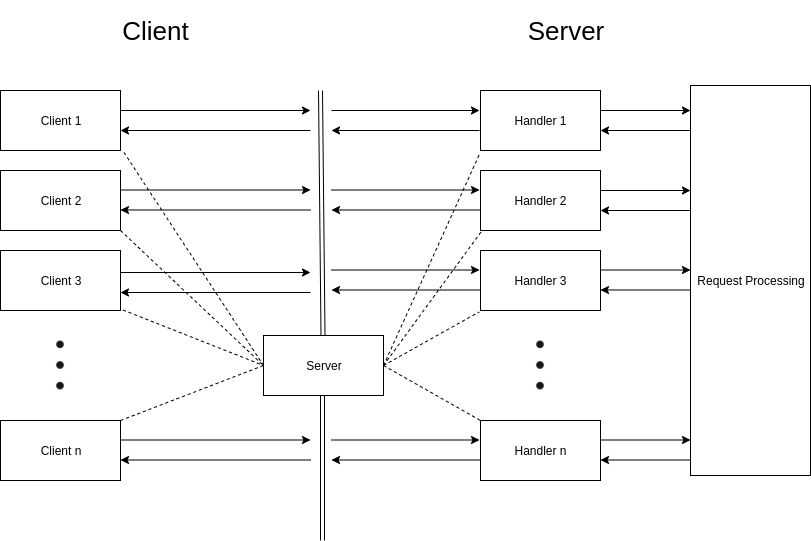
\includegraphics[width=\textwidth]{multiclientdiagram.png}
		\caption{Multi-client server working diagram}
	\end{figure}	
	
	As seen in the previous diagram, each client is able to connect, send and receive data only through a gateway. Represented by the dashed line each client will send a connection request to which the server will respond by creating a child process that will be in charge of serving the client (client handler as is the case).\\
	
	It is important to note that the server gateway will be the main thread of the server program. The main thread is in charge of only accepting any incoming connections from any client only if it connects to the corresponding port that the main thread will be constantly listening to.\\
	
	Once the connection is set, the child process created by the main server thread will be able to send and receive data to and from the client process. This let's us have a direct connection to the client while keeping the main server thread less bussy as possible.\\
	
	Something important to note is that the Request Processing block is represented as being accessed by every client handler. This means that each handler will run a copy of the request processing block, wait for a return value from the process, return to the handler and send the resulting data back to the corresponding client.\\
	
	\section{Image Filtering: Understanding}
	
	Image processing is something seen constantly from social media to more advanced algorithms that filter a given image to obtain significant data from it. For instance, if one has a very noisy image, one can apply a low-pass filter to the whole image to obtain a more smooth looking one. There are many other filters that can be applied to an image and its implementations are bounded by nothing less than imagination and what the problem requires.\\
	
	\vfill
	
	\begin{figure}[h]
		\centering
		\begin{subfigure}{.47\textwidth}
			\centering
			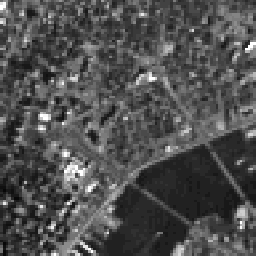
\includegraphics[width=5cm]{originalLOWPASS.png}
			\caption{Original Image}
		\end{subfigure}%		
		{\LARGE$\xrightarrow{low-pass}$}%
		\begin{subfigure}{.47\textwidth}
			\centering
			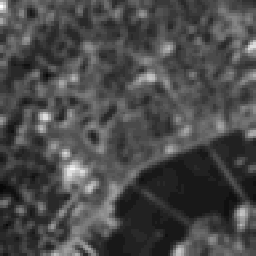
\includegraphics[width=5cm]{smoothLOWPAS.png}
			\caption{Filtered Image}
		\end{subfigure}

		\caption{Low-pass filter application to an image}
	\end{figure}	
	
	For this particular project, three filters where implemented: blur, grayscale and edge detection. One way to represent a filter being applied to an image is by thinking of an image as a matrix of numbers; each index location of the matrix represents a single pixel, each with a certain ARGB or RGBA value (depending on the system and wheter it supports the A channel):\\
	
	\begin{itemize}
		\item A: Alpha channel; represents the opacity of the image.
		\item R: Red channel; represents how much red is present in an image.
		\item G: Green channel; represents how much green is present in an image.
		\item B: Blue channel; represents how much blue is present in an image.
	\end{itemize}
	
	
	\begin{figure}[h]
		\begin{center}
			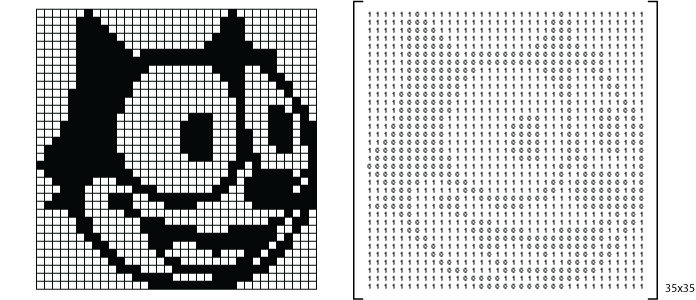
\includegraphics[width=15cm]{sample-matrix.png}
		\end{center}
		\caption{Image to matrix representation}
	\end{figure}
	
	
	
	As seen in the previous image, the ARGB values can be represented as integer or float values. For figure 3, the case would be an image of size 35 by 35 pixels consisting of only 1s and 0s where 1 is white and 0 is black. Such representations let us apply certain operations to the image matrix, seeing an image as an input signal where one could apply image convolution to such signal or any other applications required by the filter itself to obtain certain characteristics of an image or something different entirely. 
	
	\subsection{Blur}
	
	The blur method applies a blur window, which corresponds to the neighbouring pixels of a single one. How this works is we get the added value of all the RGB values of each pixel in the blur window. Once the RGB values are set, we will divide them by the number of pixels in the blur window, and the result will be stored in a single pixel on the destination image file. This can be seen in the next figure:
	
	\begin{figure}[H]
		\centering
		\begin{subfigure}{.47\textwidth}
			\centering
			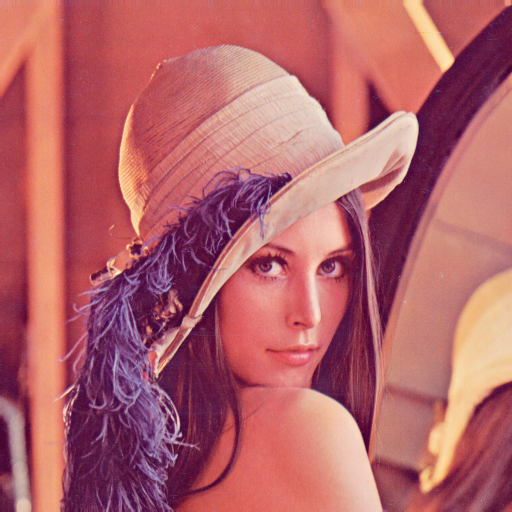
\includegraphics[width=5cm]{Lenna.png}
			\caption{Original Image}
		\end{subfigure}%		
		{\LARGE$\xrightarrow{blur}$}%
		\begin{subfigure}{.47\textwidth}
			\centering
			
\includegraphics[width=5cm]{jv_blur_Lenna.png}
			\caption{Filtered Image}
		\end{subfigure}

		\caption{Blur filter application to Lenna.png}
	\end{figure}			
	
	\subsection{Grayscale}
	
	There are many methods for implementing a grayscale filter. The method used in this project is by simply averaging the RGB values from the source image and setting that average to each RGB values on the destination image.
	
	This can be seen by implementing the filter on the following image:	
	
	\begin{figure}[H]
		\centering
		\begin{subfigure}{.47\textwidth}
			\centering
			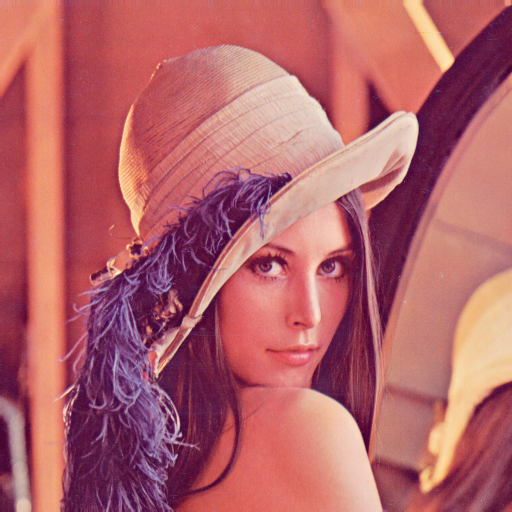
\includegraphics[width=5cm]{Lenna.png}
			\caption{Original Image}
		\end{subfigure}%		
		{\LARGE$\xrightarrow{grayscale}$}%
		\begin{subfigure}{.47\textwidth}
			\centering
			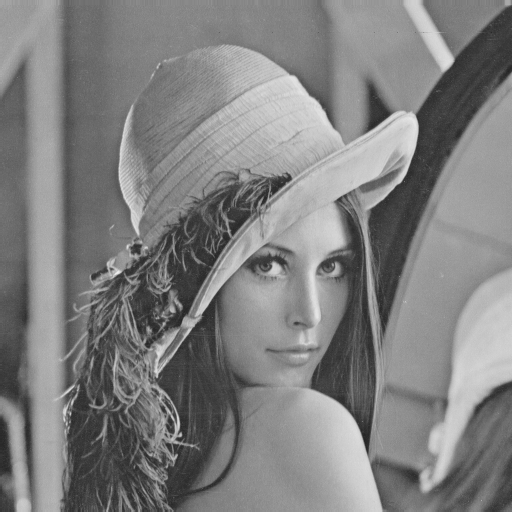
\includegraphics[width=5cm]{jv_gray_Lenna.png}
			\caption{Filtered Image}
		\end{subfigure}

		\caption{Grayscale filter application to Lenna.png}
	\end{figure}		
		
	
	\subsection{Edge detection}
	
	For the edge detection, the horizontal method was used. Although not completely efficient, it does a good job on detecting the edges of an image. Such edges are highlighted by the absolute value of the difference between the top and bottom pixels of a sliding window of a determined size. The obtained value from the difference is then compared against an empirically obtained threshold value between 0 and 1.\\ 

	\begin{figure}[h]
		\centering
		\begin{subfigure}{.47\textwidth}
			\centering
			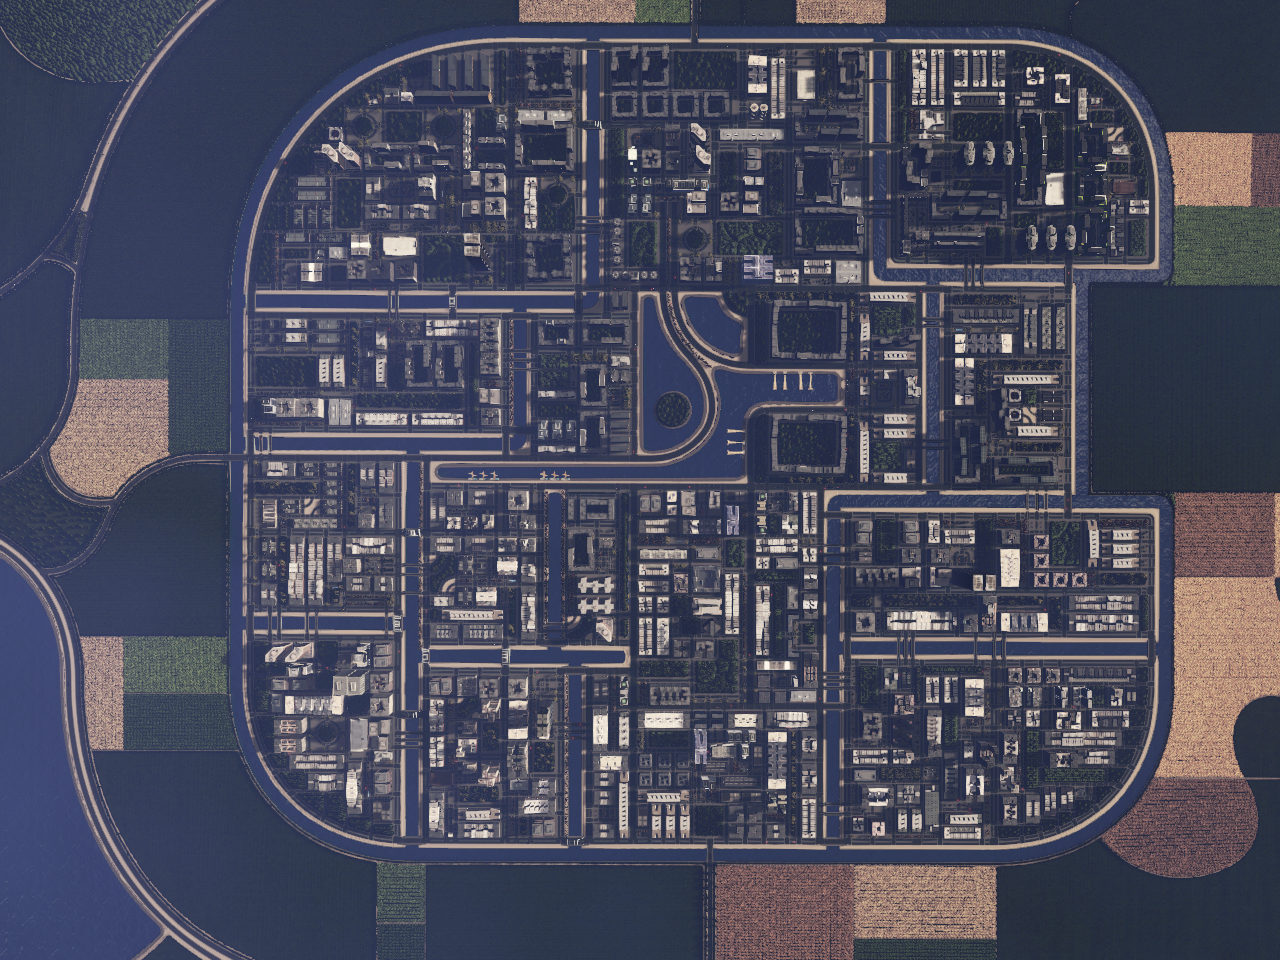
\includegraphics[width=5cm]{city2.png}
			\caption{Original Image}
		\end{subfigure}%		
		{\LARGE$\xrightarrow{edge}$}%
		\begin{subfigure}{.47\textwidth}
			\centering
			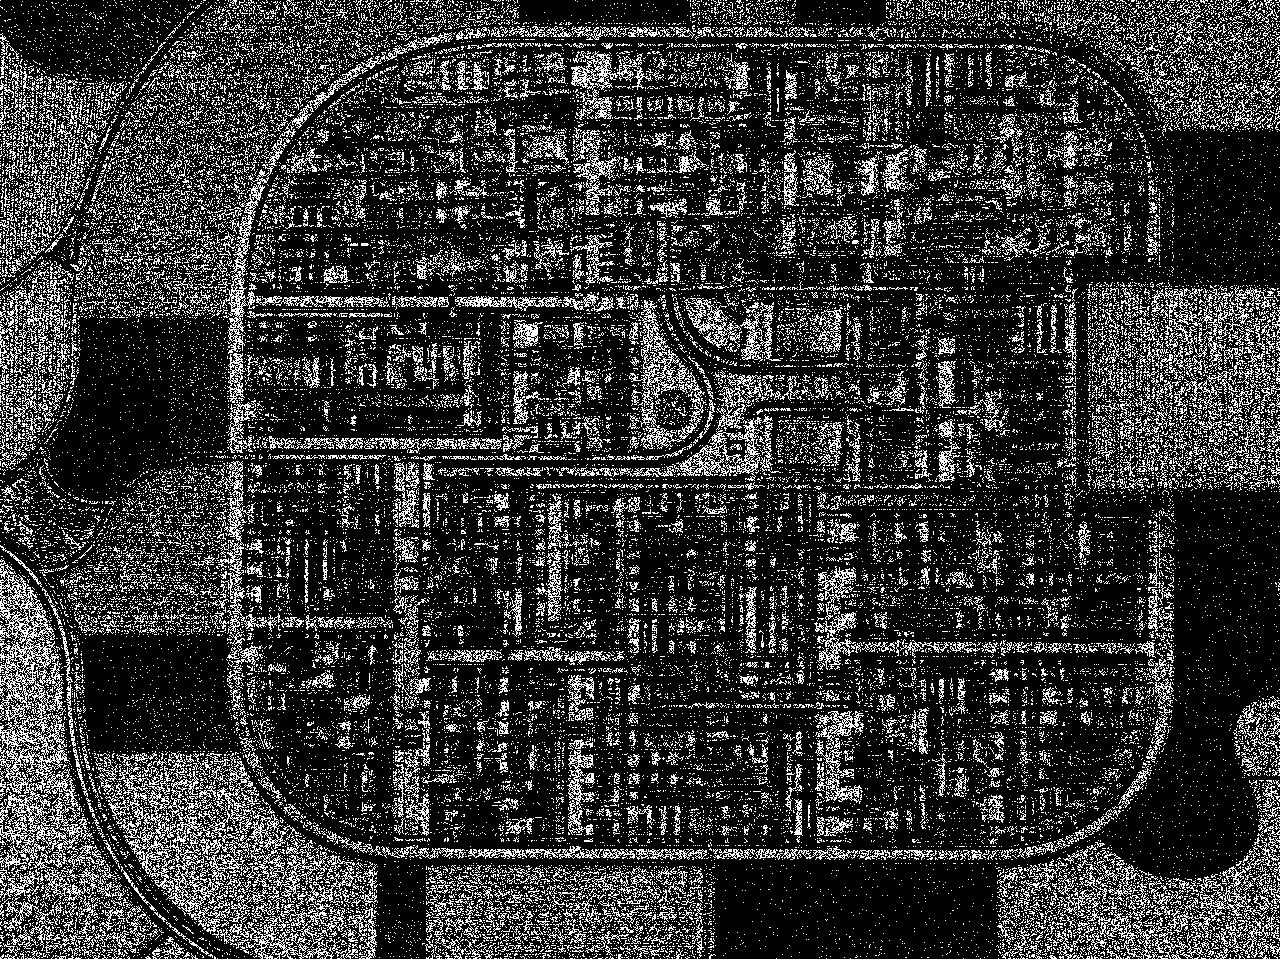
\includegraphics[width=5cm]{jv_edge_city2.png}
			\caption{Filtered Image}
		\end{subfigure}

		\caption{Edge detection filter application to a top city view}
	\end{figure}	

	In this project, the threshold value was set between 0.65 and 0.70; anything outside the threshold would be considered "white" whereas inside the threshold it would be considered black and painted respectively. Note that on this implementation the RGB values of the top and low set of pixels where averaged respectively, thus returning a somewhat grayscaled image.\\
	
	Now, this implementation works for certain images, because of how it is implemented, the algorithm struggles to work on very-defined, sharp, vertical lines. For instance, let's look at the following application of the filter:\\
	
	\begin{figure}[H]
		\centering
		\begin{subfigure}{.47\textwidth}
			\centering
			
\includegraphics[width=5cm]{coloredsquares.png}
			\caption{Original Image}
		\end{subfigure}%		
		{\LARGE$\xrightarrow{edge}$}%
		\begin{subfigure}{.47\textwidth}
			\centering
			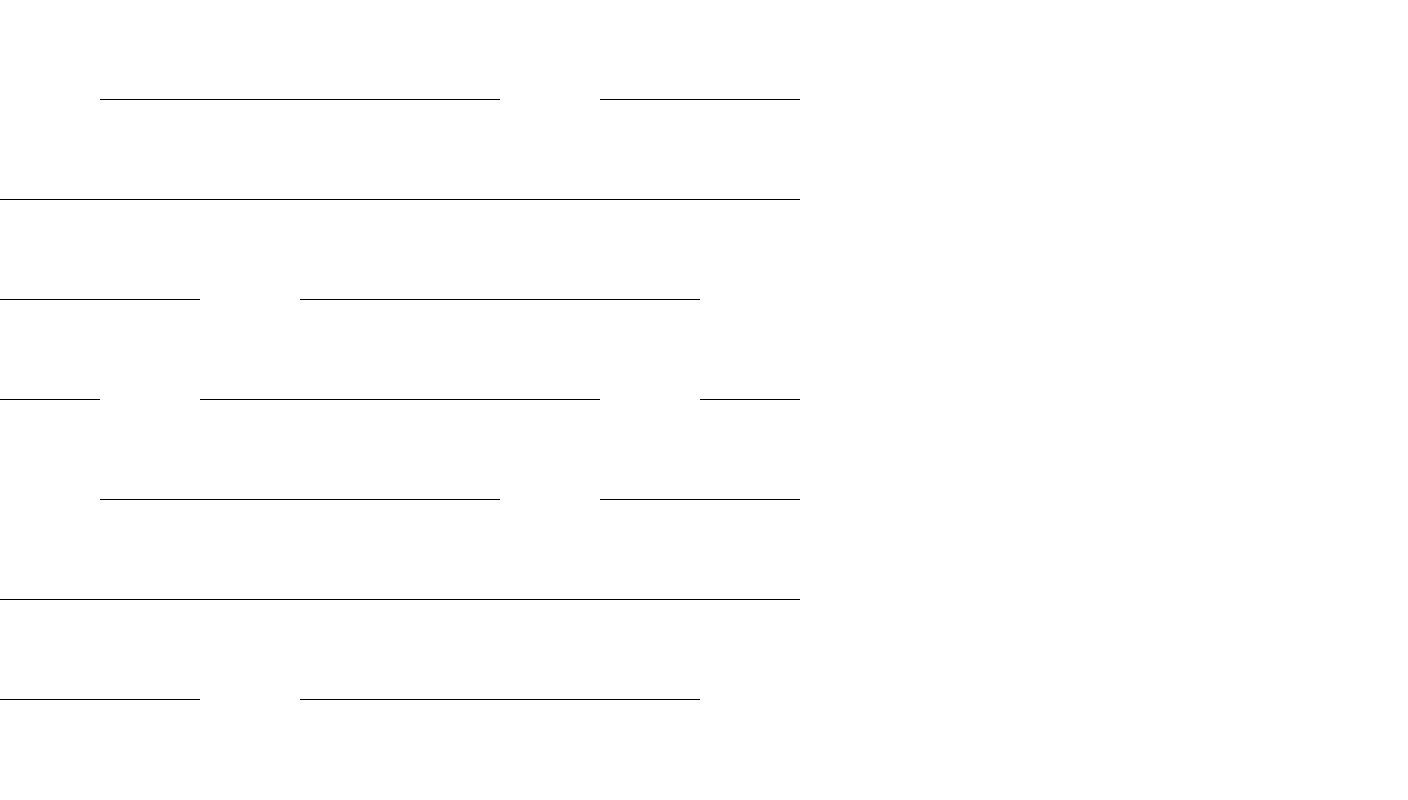
\includegraphics[width=5cm]{jv_edge_coloredsquares.png}
			\caption{Filtered Image}
		\end{subfigure}

		\caption{Edge detection filter application to colored squares}
	\end{figure}	
	
	Notice how it completely ignores any vertical lines that appear in the original image, and even tho, it fails to detect some horizontal lines as well. Even if it worked fairly well on Figure 5, we see a lack of efficiency and correctness on the algorithm. There are many other algorithms that can implement a better, more efficient, solution, but for this project the implemented algorithm will suffice. 
	
	\section{Paradigm Exploration}	
	
	For the pardigm exploration one must define which and how a given paradigm works for the wrapped solution from the previous sections (multiple-client server and image filtering). Through Java's high concurrency objects as well as the many interfaces they provide, mainly the Runnable implementation and the fork-join framework, which includes the RecursiveAction.\\
	
	This high-concurrency objects and frameworks let's us implement the communication for multiple clients, each with a single thread to work on the server side (child processes created by the server). This as well let's us apply the filters through the java fork-join framework which implements a pool of threads able to work on a single element (in this case an image) and return the result of their work in the corresponding position, as this method does not return a value per se, it stores the result of applying the filter of a source image to a destination path which the client handler will reference to retrieve the resulting image file.
	
	\section{Technology Implementation}

	In this section I'll go directly to how the application works. First, let's explore what the source directory from the client looks like at the start.
		
	\begin{figure}[H]
		\centering
		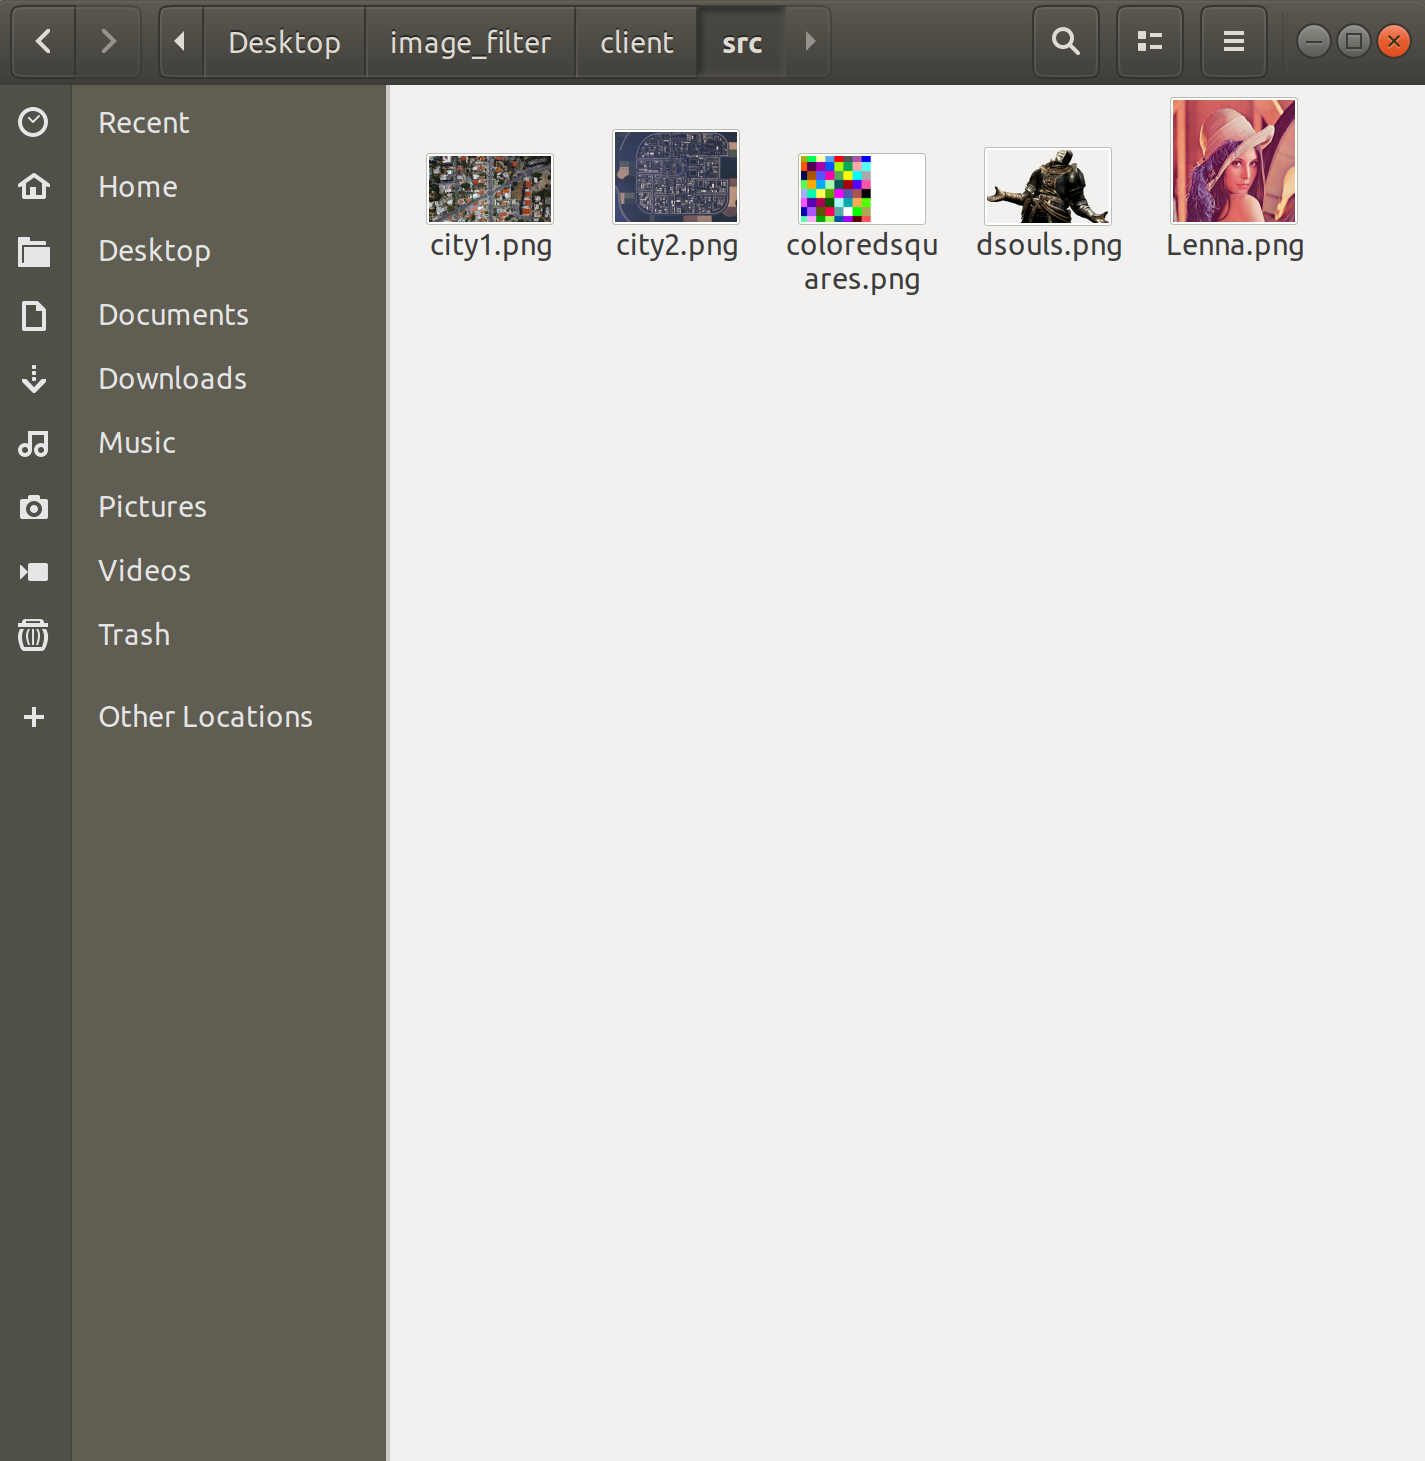
\includegraphics[width=\textwidth]{clientsrc.png}
		\caption{Single client directory}
	\end{figure}		
	
	Now that we have stored a number of images inside the source directory, let's jump to the destination directory, which as of now should be empty to demonstrate the working application.
	
	\begin{figure}[H]
		\centering
		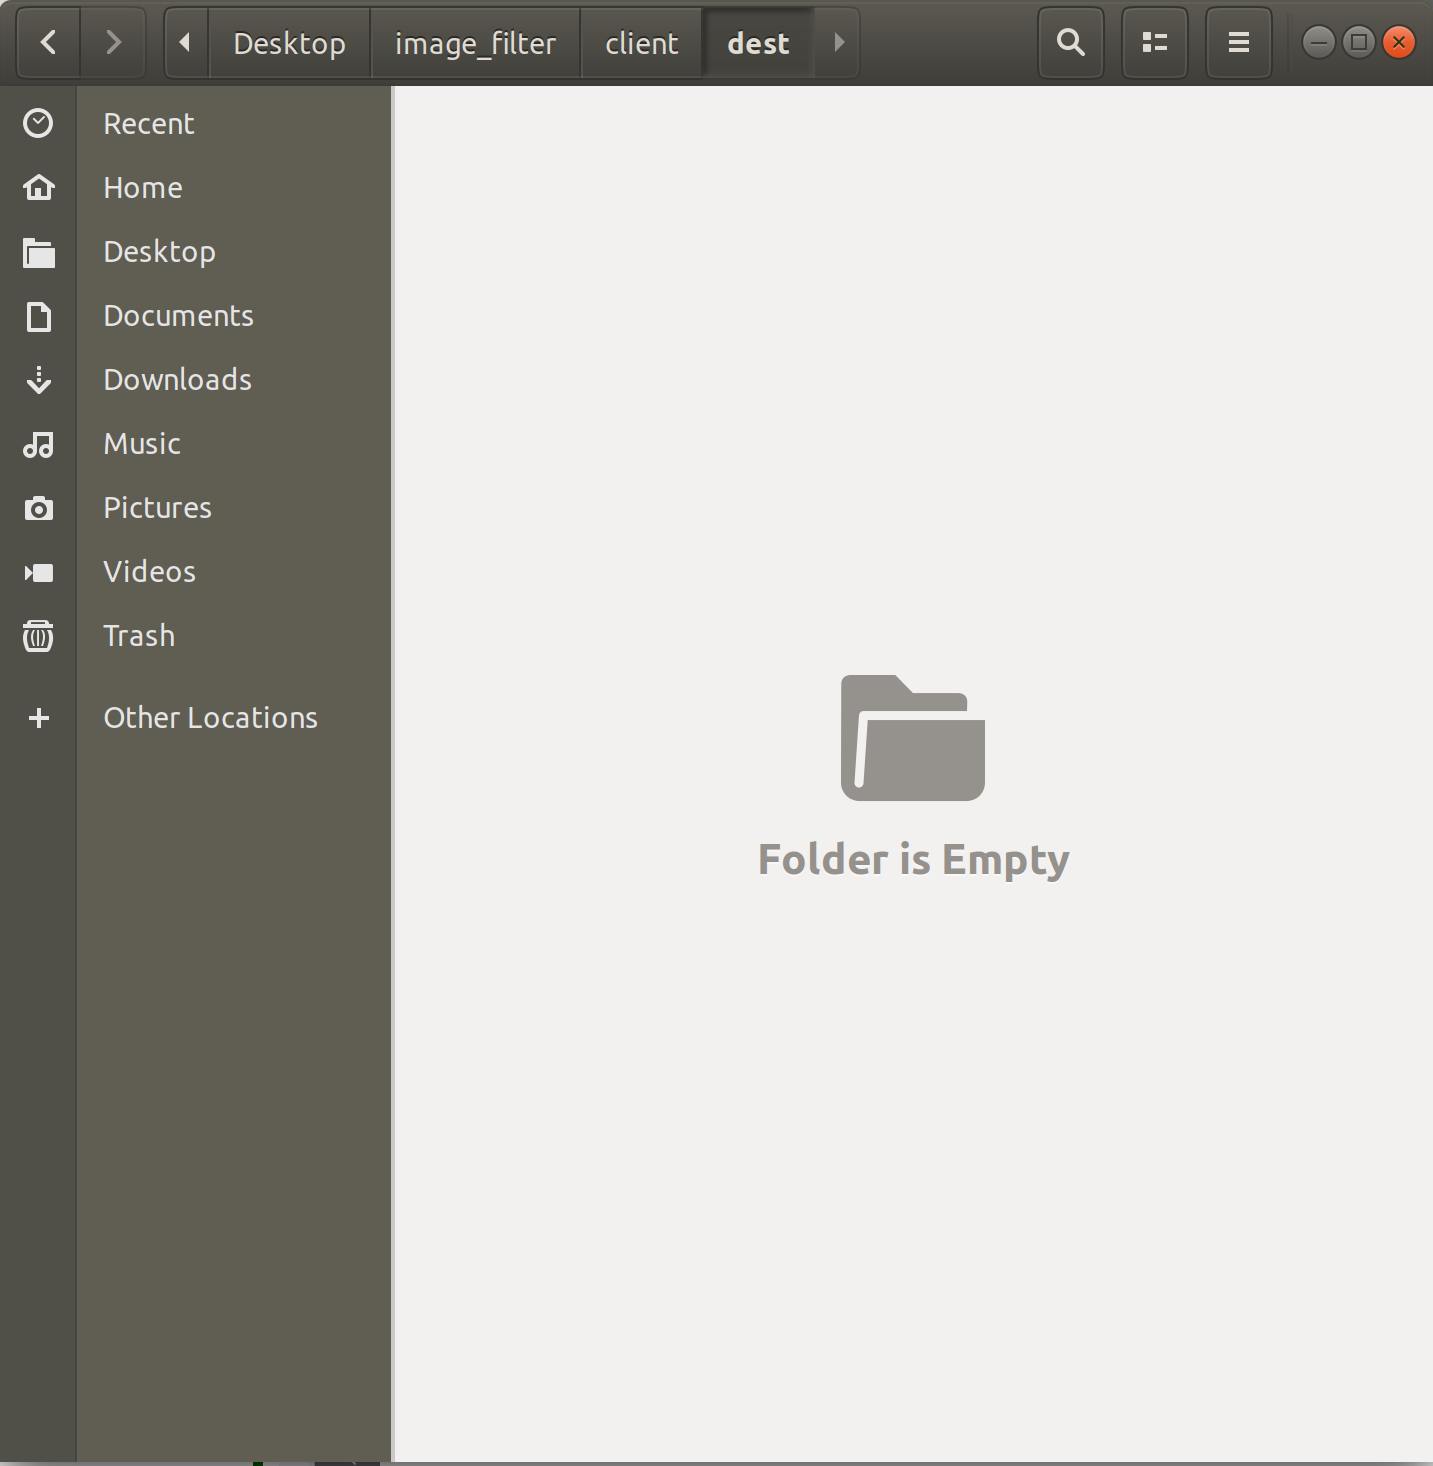
\includegraphics[width=\textwidth]{emptydirclient.png}
		\caption{Empty client destination directory. Resuls will be stored here}
	\end{figure}	
	
	Once that is set, one has to run the application. Starting from the server side, we have to run the application there before any client can connect to it. So we jump to the server side an run the application (recompile if necessary) with "java Server". The starting promt should look like this:\\
	
	
	\begin{figure}[H]
		\centering
		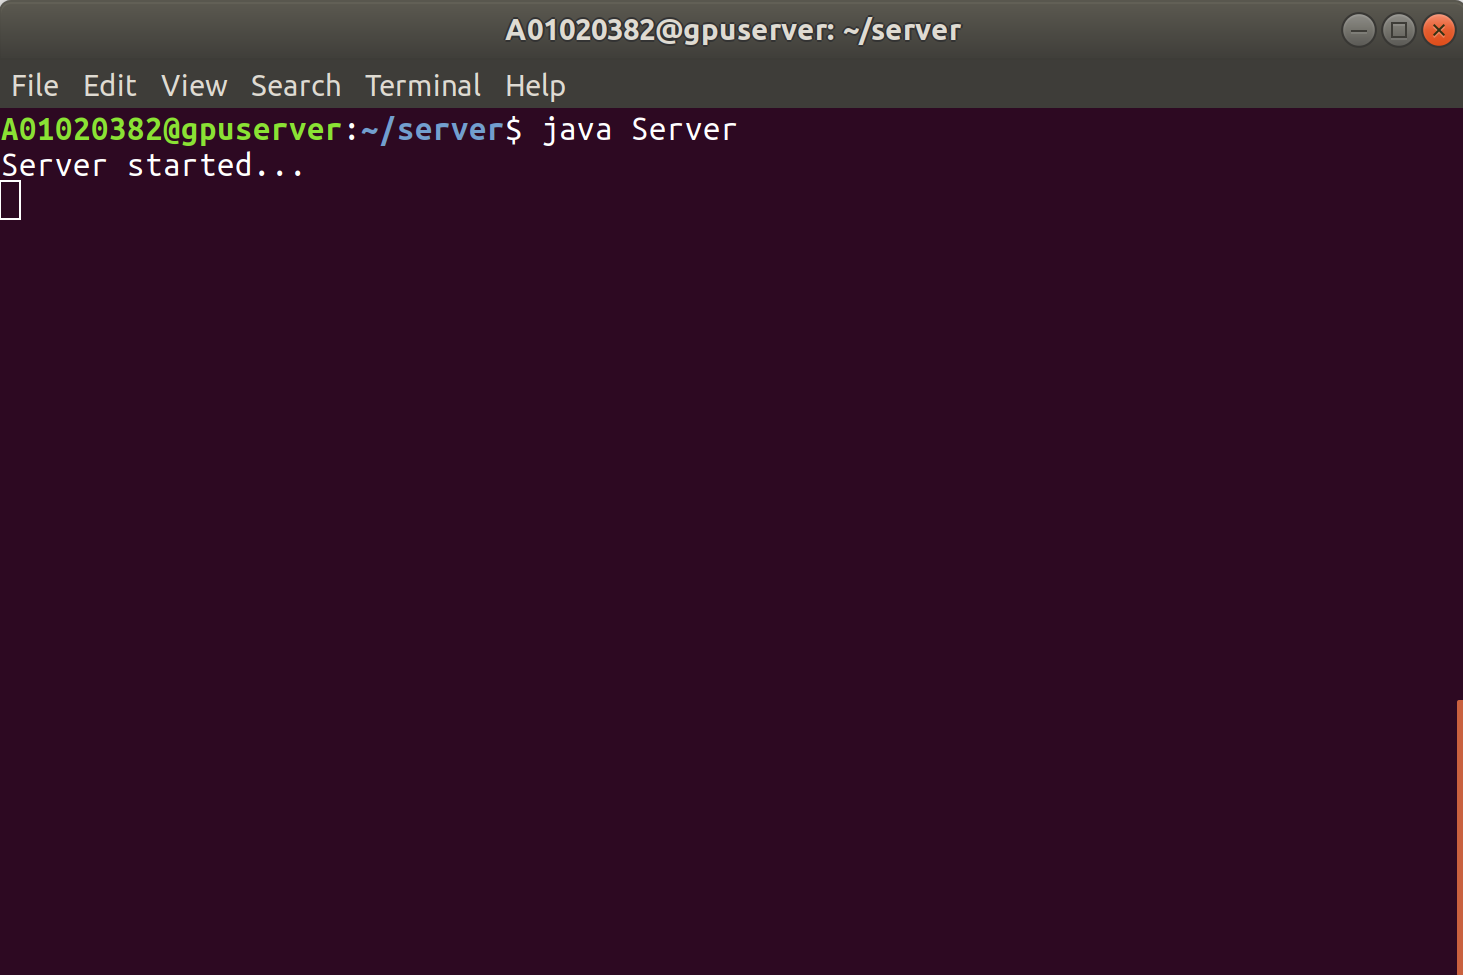
\includegraphics[width=\textwidth]{serverinit.png}
		\caption{Server starting promt}
	\end{figure}	
	
	
	Going back to the main client directory, we have to recompile (if necessary) and run the Client application (java Client). Once it's running, a message will promt and ask the user to imput certain parameters defined in the message promt. 
	
	\begin{figure}[H]
		\centering
		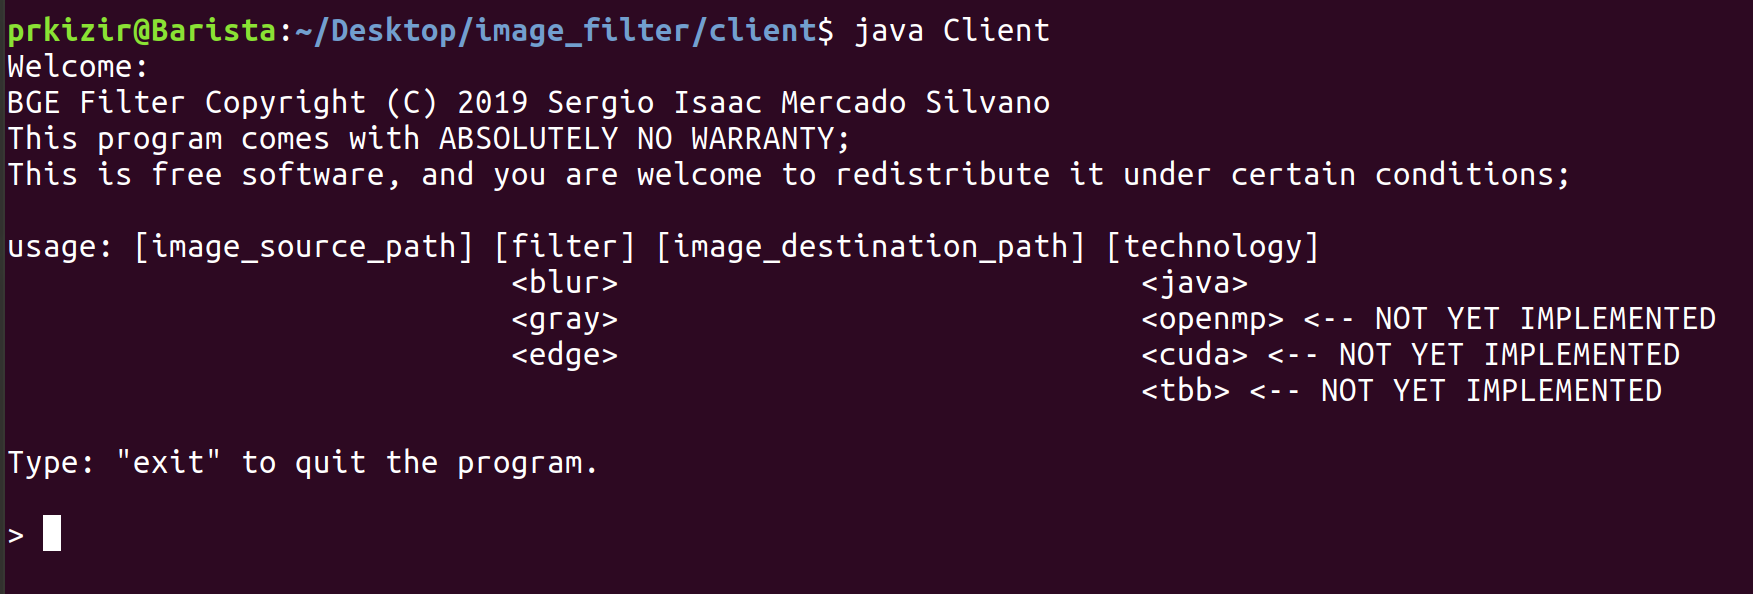
\includegraphics[width=\textwidth]{clientinit.png}
		\caption{Client starting promt}
	\end{figure}	
	
	Once the client connects this should appear on the server side, indicating that a client has connected to the server itself and shows the client's ip address.
	
	\begin{figure}[H]
		\centering
		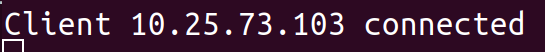
\includegraphics[width=\textwidth]{clientconnected.png}
		\caption{Client with ip address 10.25.73.103 connected}
	\end{figure}	
	
	On the client side we may request multiple filters to multiple images, passing the necessary arguments to the command line as such:
	
	\begin{figure}[H]
		\centering
		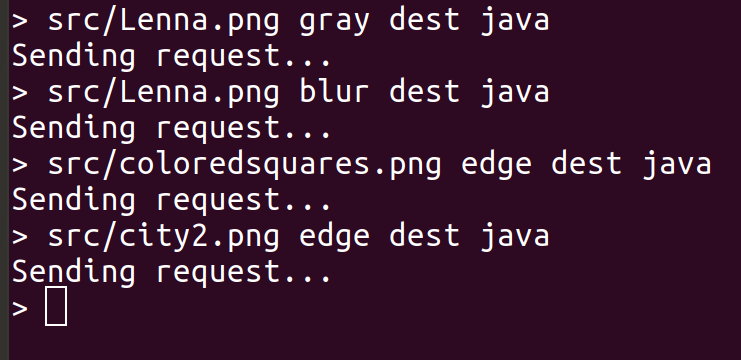
\includegraphics[width=\textwidth]{requestsclient.png}
		\caption{Multiple client requests to the server; results will be stored on the "dest" directory}
	\end{figure}	
	
	After the request is processed, the resulting image will be stored to where the client requested \textbf{relative} to where the user started the Client process. Because the other technologies are not yet implemented, I used java on the test cases; the other technologies will be implemented on further revisions. 
	
	Now if we jump back to the client destination directory, we will see that new images have been added.
	
	\begin{figure}[H]
		\centering
		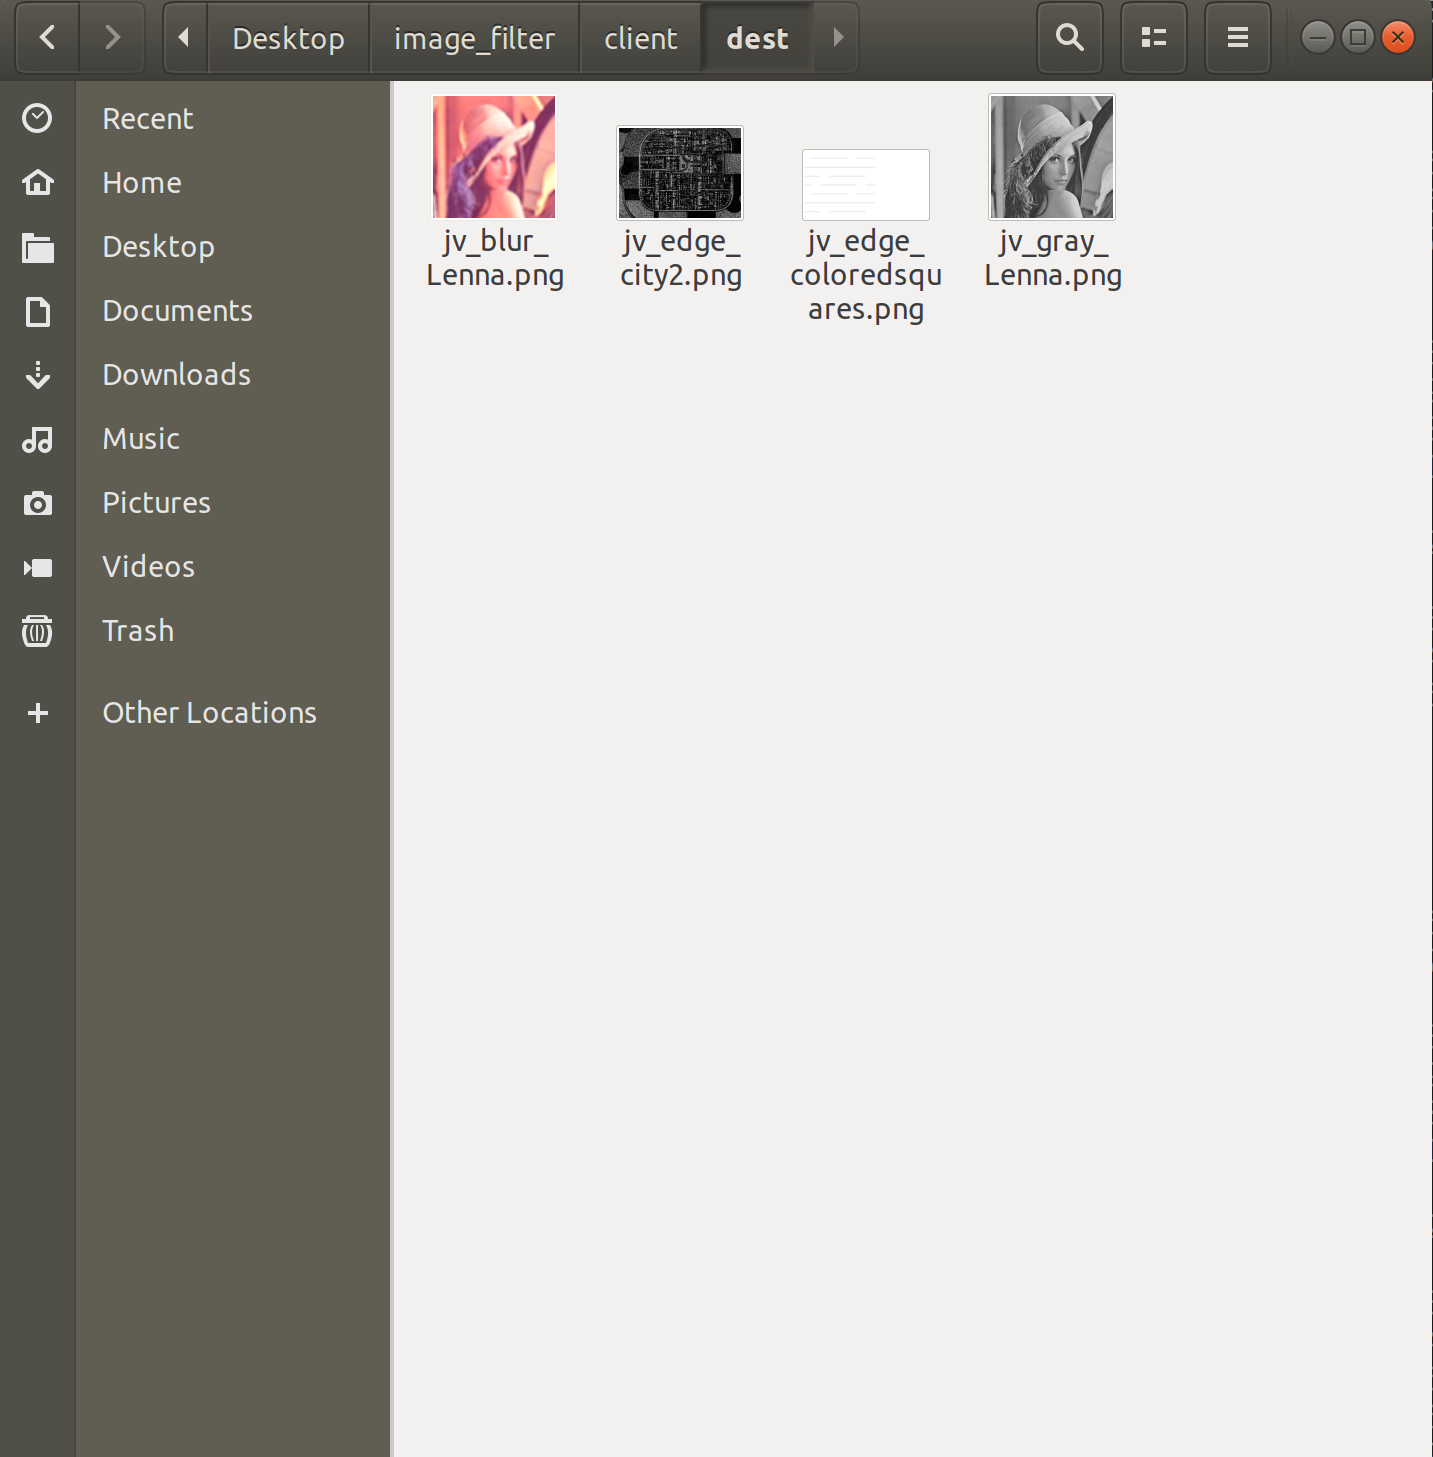
\includegraphics[width=\textwidth]{destfilled.png}
		\caption{Destination directory now with the requested images}
	\end{figure}	
	
	For the naming convention, I used the technology implemented for the filtering itself, the filter applied to the image and the original name of the image.
	
	Finally, once the client is done, it may type the "exit" command. This will indicate that the client is finished and wishes to disconnect from the server. The client process will then close its socket connections to the child process "forked" by the main server thread and indicate it has disconnected. This is visible on both sides of the application, as seen in figure.
	
	\begin{figure}[H]
		\centering
		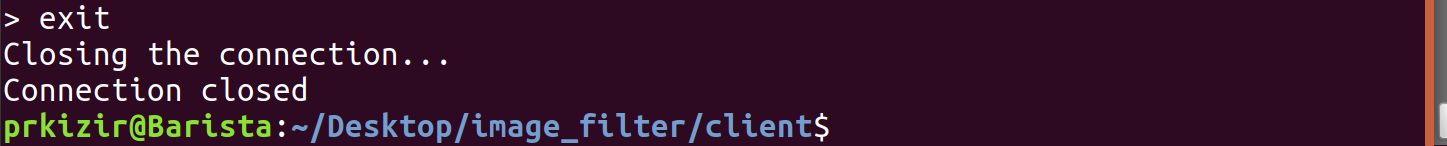
\includegraphics[width=\textwidth]{exitclient.png}
		\caption{Client side}
	\end{figure}	
	
	\begin{figure}[H]
		\centering
		
\includegraphics[width=\textwidth]{clientdisconnected.png}
		\caption{Server side}
	\end{figure}	
	
	
	\section{Applications}

	Within the previous sections we saw how to apply filters to images on a client-server basis. How does this all come together? For starters, in the field of robotics, image processing is key to many applications and with many other filters that could be applied to an image, the uses are greatly enhanced by the developer.\\
	
	For a multi-client server, such applications would come in the form of a unified network of machines that could map, with the help of computer vision, a whole area just by border detection and sending that information to a server that could put the pieces together.\\
	
	The implementation of this project was mostly directed toward users that would select an image manually and apply one (or all) of the filters available; subsequently the users would receive the filtered image they requested.\\

	\section{Conclussions}
	
	Although a simple implementation, this project could be expanded using not only Java's high concurrency objects and frameworks, but other technologies as well that tackle another kind of paradigm such as full parallelism, which greatly enhances image processing and thus increasing the response time from the server.\\
	
	It is interesting how image processing works and the many applications it entitles. It is up to us, the developers, to indulge oneself in the vast world of image processing. Looking at how this may apply to my field of study I profoundly see great applications in robotics and computer vision that would greatly change the way we see the Universe that surrounds us.
		
	\section{Bibliography}
	
	
	[1] C. Saravanan (2010). Color  Image to Grayscale Image Conversion. Retrieved from \url{https://ieeexplore.ieee.org/stamp/stamp.jsp?tp=&arnumber=5445596&fbclid=IwAR1EgoKwX5CnBjdJQLrgmHkPzlmUKyQvZK35JP7GaRMgt2HXUBtrC4h3BYE&tag=1}\\
	
	[2] Introcomputing (n..d). Grayscale Images. Retrieved from \url{https://introcomputing.org/image-6-grayscale.html?fbclid=IwAR0E8mxXjILrPbYgxgdtetfgdf2_piGEpXAc6OQhZhpgus4MYEiat8IyA9I}\\
	
	[3] B. Poornima, Y. Ramadevi, T. Sridevi (2011). Threshold Based Edge Detection Algorithm. Retrieved from \url{http://ijetch.org/papers/260-T754.pdf?fbclid=IwAR3qX0VZJMqMxe5RodFxJM7QK4rXKWj-OHE29homJzEwlR27NpOj_r80zX4}\\
	
	[4] You-yi Zheng, Ji-lai Rao, Lei Wu, et. al. (2010). Edge Detection Methods in Digital Image Processing. Retrieved from \url{https://ieeexplore.ieee.org/stamp/stamp.jsp?tp=&arnumber=5593576&fbclid=IwAR2rIoQ70Uq63shHmBwwlO0mYrun1aZYb9anzHsQGkAilB4q-GfDx1E49Xg}\\
	
	[5] user: Packt-Pub (n.d.). Building a Java Edge Detection Application. Retrieved from \url{https://medium.com/javarevisited/building-a-java-edge-detection-application-6147b68e5d79}\\
		
	[6] IDL Online Help (2005). Filtering an Image. Retrieved from \url{https://northstar-www.dartmouth.edu/doc/idl/html_6.2/Filtering_an_Imagehvr.html?fbclid=IwAR3hdgPAXU28LdKZctmNI6JI18w_dJ9X1ko09TBdH9-H_8zbflQlKeUzVC0#wp1022750}\\
	
	[7] (n.a) (n.d). Chapter 4. Image Filtering. Retrieved from \url{http://www.cse.usf.edu/~r1k/MachineVisionBook/MachineVision.files/MachineVision_Chapter4.pdf?fbclid=IwAR1qzygXluRKIKnm0t0RTB8uhsjJHFtPJXZEJ5fvKWFzWWnwpEYd_FhXFGg}\\
	
	[8] Geeks for Geeks (n.d.). Introducing Threads in Socket Programming in Java. Retrieved from \url{https://www.geeksforgeeks.org/introducing-threads-socket-programming-java/?fbclid=IwAR3qX0VZJMqMxe5RodFxJM7QK4rXKWj-OHE29homJzEwlR27NpOj_r80zX4}\\
	
	[9]	Geeks for Geeks (n.d). Digital Image Processing Basics. Retrieved from \url{https://www.geeksforgeeks.org/digital-image-processing-basics/?fbclid=IwAR1DqGltCVK4AeQchqvB0rQHWLMc3ayRs_0cxDqdDD52ooNbCelDNmwuSms}\\
	
	[10] Daniel Shiffman (2008). Images and Pixels. Retrieved from \url{https://processing.org/tutorials/pixels/?fbclid=IwAR2po0c9tc3QPYgagWEWcQ5MQr1Vq0extRHtNWz2oRIuuMOI6gXbpH9ZzGs}\\
	
	[11] Alvin Alexander (2016). Java exec - execute system processes with Java ProcessBuilder and Process. Retrieved from \url{https://alvinalexander.com/java/java-exec-processbuilder-process-1}\\
	
\end{document}